% TikZ diagram: OpenMP vs MPI Game Modes Comparison
% Compile with: pdflatex openmp-vs-mpi-modes.tex

\documentclass[tikz,border=10pt]{standalone}
\usepackage{tikz}
\usetikzlibrary{shapes,arrows,positioning,fit,backgrounds,patterns}

\begin{document}
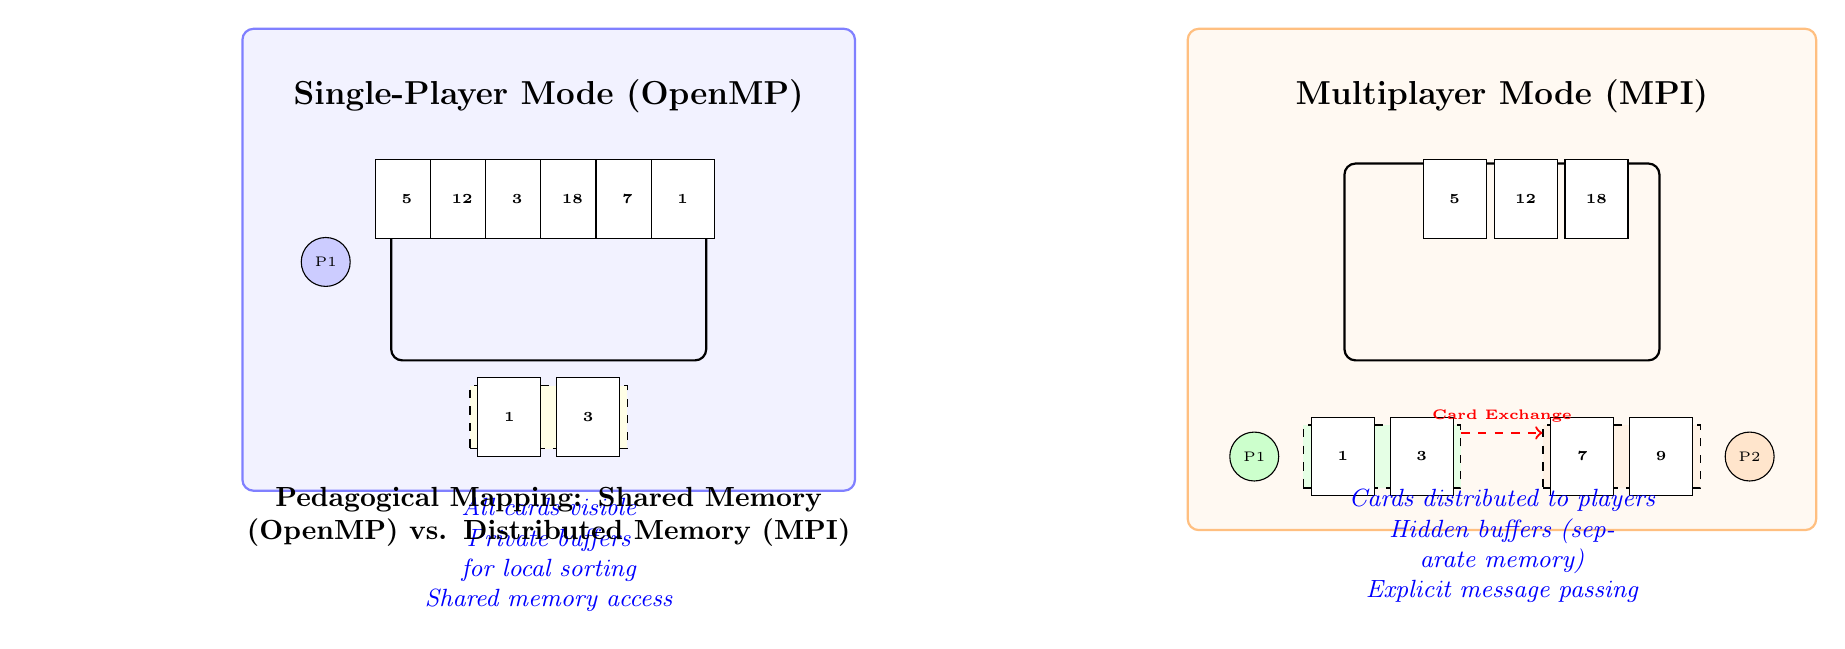
\begin{tikzpicture}[
    node distance=1cm,
    card/.style={rectangle, draw, fill=white, minimum width=0.8cm, minimum height=1cm, font=\tiny\bfseries},
    container/.style={rectangle, draw, thick, rounded corners, minimum width=4cm, minimum height=2.5cm},
    buffer/.style={rectangle, draw, dashed, fill=yellow!10, minimum width=2cm, minimum height=0.8cm},
    player/.style={circle, draw, fill=blue!20, minimum size=0.6cm, font=\tiny},
    label/.style={font=\bfseries\large},
    concept/.style={font=\small\itshape, text=blue}
]

% OpenMP Mode (Left Side)
\node[label] (openmp-title) {Single-Player Mode (OpenMP)};

\node[container, below=0.5cm of openmp-title, label=below:\textbf{Shared Container}] (openmp-container) {};

% Cards in shared container
\foreach \i/\num in {1/5, 2/12, 3/3, 4/18, 5/7, 6/1} {
    \node[card] at ([xshift=\i*0.7cm-2.5cm, yshift=0.8cm]openmp-container) {\num};
}

% Private buffers
\node[buffer, below=0.3cm of openmp-container, label=below:Private Buffer] (openmp-buffer) {};
\node[card] at ([xshift=-0.5cm]openmp-buffer) {1};
\node[card] at ([xshift=0.5cm]openmp-buffer) {3};

% Player representation
\node[player, left=0.5cm of openmp-container] (openmp-player) {P1};

% Concepts
\node[concept, below=0.5cm of openmp-buffer, text width=4cm, align=center] {
    All cards visible\\
    Private buffers for local sorting\\
    Shared memory access
};

% MPI Mode (Right Side)
\node[label, right=6cm of openmp-title] (mpi-title) {Multiplayer Mode (MPI)};

\node[container, below=0.5cm of mpi-title, label=below:\textbf{Shared Container}] (mpi-container) {};

% Fewer cards in shared container (some distributed)
\foreach \i/\num in {1/5, 2/12, 3/18} {
    \node[card] at ([xshift=\i*0.9cm-1.5cm, yshift=0.8cm]mpi-container) {\num};
}

% Player 1 buffer
\node[buffer, below left=0.8cm and -1.5cm of mpi-container, fill=green!10, label=below:Player 1] (mpi-buffer1) {};
\node[card] at ([xshift=-0.5cm]mpi-buffer1) {1};
\node[card] at ([xshift=0.5cm]mpi-buffer1) {3};

% Player 2 buffer
\node[buffer, below right=0.8cm and -1.5cm of mpi-container, fill=orange!10, label=below:Player 2] (mpi-buffer2) {};
\node[card] at ([xshift=-0.5cm]mpi-buffer2) {7};
\node[card] at ([xshift=0.5cm]mpi-buffer2) {9};

% Players
\node[player, left=0.3cm of mpi-buffer1, fill=green!20] (mpi-player1) {P1};
\node[player, right=0.3cm of mpi-buffer2, fill=orange!20] (mpi-player2) {P2};

% Message passing arrow
\draw[->, thick, red, dashed] ([yshift=0.3cm]mpi-buffer1.east) --
    node[above, font=\tiny\bfseries] {Card Exchange} ([yshift=0.3cm]mpi-buffer2.west);

% Concepts
\node[concept, below=1.5cm of mpi-container, text width=4cm, align=center] {
    Cards distributed to players\\
    Hidden buffers (separate memory)\\
    Explicit message passing
};

% Bottom comparison
\node[below=4.5cm of openmp-title, font=\bfseries, text width=13cm, align=center] {
    Pedagogical Mapping: Shared Memory (OpenMP) vs. Distributed Memory (MPI)
};

% Background boxes
\begin{scope}[on background layer]
    \node[fit=(openmp-title)(openmp-container)(openmp-buffer)(openmp-player),
          fill=blue!5, draw=blue!50, thick, rounded corners, inner sep=15pt] {};
    \node[fit=(mpi-title)(mpi-container)(mpi-buffer1)(mpi-buffer2)(mpi-player1)(mpi-player2),
          fill=orange!5, draw=orange!50, thick, rounded corners, inner sep=15pt] {};
\end{scope}

\end{tikzpicture}
\end{document}
